% Memoria (3 caras, doble columna) — plantilla uc3mmaster. Compilar desde esta carpeta: latexmk -pdf memoria.tex
% Todas las cifras vienen de ../numeros.tex y las filas de tablas de ../tablas.tex (generados por ../analisis.py).
\documentclass[memoria,twocolumn]{uc3mmaster}
\newgeometry{top=1.7cm,bottom=1.6cm,left=1.45cm,right=1.45cm,headheight=13pt,headsep=8pt,footskip=16pt}
\setlength{\columnsep}{0.6cm}
\usetikzlibrary{arrows.meta,positioning}
\definecolor{azulm}{HTML}{2E6DB4}\definecolor{naranjam}{HTML}{D9731A}
\definecolor{verdem}{HTML}{2F9467}\definecolor{grism}{HTML}{5A6772}
% Generado por analisis.py: NO editar a mano.
\newcommand{\nDatasets}{12}
\newcommand{\nParticiones}{5}
\newcommand{\cambioRL}{$-$14{,}6\,\%}
\newcommand{\dsRL}{11/12}
\newcommand{\pRL}{$0{,}027$}
\newcommand{\pSinHolmRL}{$0{,}003$}
\newcommand{\vsEstRL}{$-$13{,}1\,\%}
\newcommand{\pVsEstRL}{$0{,}027$}
\newcommand{\peorRL}{$+$1{,}2\,\%}
\newcommand{\peorDsRL}{kin8nm}
\newcommand{\cambioKNN}{$-$21{,}2\,\%}
\newcommand{\dsKNN}{9/12}
\newcommand{\pKNN}{$0{,}161$}
\newcommand{\pSinHolmKNN}{$0{,}027$}
\newcommand{\vsEstKNN}{$-$10{,}0\,\%}
\newcommand{\pVsEstKNN}{$0{,}386$}
\newcommand{\peorKNN}{$+$28{,}5\,\%}
\newcommand{\peorDsKNN}{kin8nm}
\newcommand{\cambioArbol}{$-$0{,}6\,\%}
\newcommand{\dsArbol}{5/12}
\newcommand{\pArbol}{$1{,}000$}
\newcommand{\pSinHolmArbol}{$0{,}910$}
\newcommand{\vsEstArbol}{$-$0{,}7\,\%}
\newcommand{\pVsEstArbol}{$1{,}000$}
\newcommand{\peorArbol}{$+$6{,}7\,\%}
\newcommand{\peorDsArbol}{kin8nm}
\newcommand{\cambioRF}{$+$0{,}3\,\%}
\newcommand{\dsRF}{5/12}
\newcommand{\pRF}{$1{,}000$}
\newcommand{\pSinHolmRF}{$0{,}733$}
\newcommand{\vsEstRF}{$+$0{,}3\,\%}
\newcommand{\pVsEstRF}{$1{,}000$}
\newcommand{\peorRF}{$+$12{,}4\,\%}
\newcommand{\peorDsRF}{kin8nm}
\newcommand{\cambioMedio}{$-$9{,}5\,\%}
\newcommand{\sinKinRL}{$-$15{,}9\,\%}
\newcommand{\pSinKinRL}{$0{,}004$}
\newcommand{\sinKinKNN}{$-$24{,}6\,\%}
\newcommand{\pSinKinKNN}{$0{,}021$}
\newcommand{\sinKinArbol}{$-$1{,}3\,\%}
\newcommand{\pSinKinArbol}{$1{,}000$}
\newcommand{\sinKinRF}{$-$0{,}8\,\%}
\newcommand{\pSinKinRF}{$1{,}000$}
\newcommand{\sinKinMedio}{$-$11{,}2\,\%}
\newcommand{\maxRL}{$-$59{,}6\,\%}
\newcommand{\maxDsRL}{cpu\_small}
\newcommand{\maxKNN}{$-$58{,}7\,\%}
\newcommand{\maxDsKNN}{california}
\newcommand{\maxArbol}{$-$9{,}8\,\%}
\newcommand{\maxDsArbol}{space\_ga}
\newcommand{\maxRF}{$-$11{,}7\,\%}
\newcommand{\maxDsRF}{space\_ga}
\newcommand{\maxMaeOrig}{6{,}25}
\newcommand{\maxMaeP}{2{,}52}
\newcommand{\dimMedia}{83\,\%}
\newcommand{\origMedia}{4{,}9}
\newcommand{\compMedia}{2{,}2}
\newcommand{\fracComp}{93\,\%}
\newcommand{\fracElim}{43\,\%}
\newcommand{\siempreMenor}{sí}
\newcommand{\segMediana}{292}
\newcommand{\segMax}{438}
\newcommand{\cribCasos}{14}
\newcommand{\cribP}{0{,}900}
\newcommand{\cribPSeg}{199}
\newcommand{\cribPKNN}{0{,}758}
\newcommand{\cribKnn}{0{,}909}
\newcommand{\cribKnnSeg}{113}
\newcommand{\cribKnnKNN}{0{,}740}
\newcommand{\cribMinimax}{0{,}939}
\newcommand{\cribMinimaxSeg}{234}
\newcommand{\cribMinimaxKNN}{0{,}824}
\newcommand{\cribFamilia}{0{,}893}
\newcommand{\cribFamiliaSeg}{121}
\newcommand{\cribFamiliaKNN}{0{,}740}
\newcommand{\cribParada}{0{,}928}
\newcommand{\cribParadaSeg}{69}
\newcommand{\cribParadaKNN}{0{,}794}
\newcommand{\cribParadaTreinta}{0{,}923}
\newcommand{\cribParadaTreintaSeg}{84}
\newcommand{\cribParadaTreintaKNN}{0{,}794}
\newcommand{\cribSeleccion}{0{,}923}
\newcommand{\cribSeleccionSeg}{95}
\newcommand{\cribSeleccionKNN}{0{,}795}
\newcommand{\ablCasos}{24}
\newcommand{\ablKnn}{$+$1{,}4\,\%}
\newcommand{\ablKnnRL}{$+$12{,}2\,\%}
\newcommand{\ablKnnKNN}{$-$3{,}2\,\%}
\newcommand{\ablKnnArbol}{$-$2{,}1\,\%}
\newcommand{\ablKnnRF}{$-$0{,}5\,\%}
\newcommand{\ablKnnDim}{0{,}83}
\newcommand{\ablSinSint}{$-$0{,}2\,\%}
\newcommand{\ablSinSintRL}{$+$0{,}2\,\%}
\newcommand{\ablSinSintKNN}{$-$1{,}4\,\%}
\newcommand{\ablSinSintArbol}{$+$0{,}5\,\%}
\newcommand{\ablSinSintRF}{$+$0{,}1\,\%}
\newcommand{\ablSinSintDim}{0{,}77}
\newcommand{\ablSinForma}{$+$4{,}1\,\%}
\newcommand{\ablSinFormaRL}{$+$14{,}1\,\%}
\newcommand{\ablSinFormaKNN}{$+$2{,}2\,\%}
\newcommand{\ablSinFormaArbol}{$+$0{,}0\,\%}
\newcommand{\ablSinFormaRF}{$+$0{,}6\,\%}
\newcommand{\ablSinFormaDim}{0{,}75}
\newcommand{\ablSinLimite}{$-$0{,}6\,\%}
\newcommand{\ablSinLimiteRL}{$+$0{,}4\,\%}
\newcommand{\ablSinLimiteKNN}{$-$1{,}3\,\%}
\newcommand{\ablSinLimiteArbol}{$-$1{,}1\,\%}
\newcommand{\ablSinLimiteRF}{$-$0{,}6\,\%}
\newcommand{\ablSinLimiteDim}{1{,}32}
\newcommand{\ablAleat}{$+$3{,}5\,\%}
\newcommand{\ablAleatRL}{$+$4{,}5\,\%}
\newcommand{\ablAleatKNN}{$+$5{,}5\,\%}
\newcommand{\ablAleatArbol}{$+$1{,}9\,\%}
\newcommand{\ablAleatRF}{$+$2{,}1\,\%}
\newcommand{\ablAleatDim}{0{,}82}
\newcommand{\ablAG}{$+$0{,}0\,\%}
\newcommand{\ablAGRL}{$+$0{,}3\,\%}
\newcommand{\ablAGKNN}{$+$0{,}7\,\%}
\newcommand{\ablAGArbol}{$-$0{,}2\,\%}
\newcommand{\ablAGRF}{$-$0{,}7\,\%}
\newcommand{\ablAGDim}{0{,}85}
\newcommand{\rangoP}{3{,}6}
\newcommand{\posP}{1}
\newcommand{\rangoPG}{4{,}0}
\newcommand{\compPGRL}{$-$15{,}7\,\%}
\newcommand{\compPGKNN}{$-$18{,}0\,\%}
\newcommand{\compPGArbol}{$+$0{,}7\,\%}
\newcommand{\compPGRF}{$+$0{,}8\,\%}
\newcommand{\rangoEstPCA}{4{,}1}
\newcommand{\compEstPCARL}{$-$1{,}8\,\%}
\newcommand{\compEstPCAKNN}{$-$12{,}4\,\%}
\newcommand{\compEstPCAArbol}{$-$0{,}6\,\%}
\newcommand{\compEstPCARF}{$-$1{,}9\,\%}
\newcommand{\rangoMLKR}{5{,}2}
\newcommand{\compMLKRRL}{$-$1{,}8\,\%}
\newcommand{\compMLKRKNN}{$-$22{,}5\,\%}
\newcommand{\compMLKRArbol}{$+$2{,}0\,\%}
\newcommand{\compMLKRRF}{$+$2{,}6\,\%}
\newcommand{\rangoPCA}{7{,}2}
\newcommand{\compPCARL}{$+$0{,}6\,\%}
\newcommand{\compPCAKNN}{$-$10{,}4\,\%}
\newcommand{\compPCAArbol}{$+$19{,}3\,\%}
\newcommand{\compPCARF}{$+$17{,}9\,\%}
\newcommand{\rangoYJMV}{4{,}3}
\newcommand{\compYJMVRL}{$+$2{,}4\,\%}
\newcommand{\compYJMVKNN}{$-$14{,}5\,\%}
\newcommand{\compYJMVArbol}{$+$1{,}5\,\%}
\newcommand{\compYJMVRF}{$+$1{,}7\,\%}
% Generado por analisis.py.
\newcommand{\filasPrincipal}{%
R. lineal & 0{,}98 & \textbf{0{,}85} & 11/12 & $0{,}027$ & $-$13{,}1\,\% & $0{,}027$\\
KNN & 0{,}88 & \textbf{0{,}79} & 9/12 & $0{,}161$ & $-$10{,}0\,\% & $0{,}386$\\
Árbol & 1{,}00 & \textbf{0{,}99} & 5/12 & $1{,}000$ & $-$0{,}7\,\% & $1{,}000$\\
RF & 1{,}00 & \textbf{1{,}00} & 5/12 & $1{,}000$ & $+$0{,}3\,\% & $1{,}000$\\
}
\newcommand{\filasDimension}{%
diabetes & 10 & 6{,}2 & 2{,}8 & 9{,}0\\
california & 8 & 5{,}0 & 2{,}0 & 7{,}0\\
concrete & 8 & 5{,}8 & 1{,}0 & 6{,}8\\
stock & 9 & 6{,}4 & 1{,}6 & 8{,}0\\
space\_ga & 6 & 2{,}8 & 2{,}2 & 5{,}0\\
sulfur & 6 & 3{,}0 & 2{,}0 & 5{,}0\\
kin8nm & 8 & 4{,}6 & 2{,}4 & 7{,}0\\
bank8FM & 8 & 3{,}6 & 3{,}4 & 7{,}0\\
puma8NH & 8 & 2{,}2 & 0{,}6 & 2{,}8\\
house\_8L & 8 & 5{,}4 & 1{,}6 & 7{,}0\\
cpu\_small & 12 & 7{,}2 & 3{,}8 & 11{,}0\\
wine\_quality & 11 & 7{,}0 & 3{,}0 & 10{,}0\\
}
\newcommand{\filasCribado}{%
\textbf{$P$: KNN+RL+árbol} & 0{,}91 & 0{,}76 & 0{,}96 & 0{,}99 & 0{,}900 & 0{,}993 & 199\\
fitness solo KNN & 0{,}96 & 0{,}74 & 0{,}97 & 0{,}99 & 0{,}909 & 0{,}992 & 113\\
fitness minimax & 0{,}94 & 0{,}82 & 0{,}99 & 1{,}01 & 0{,}939 & 1{,}012 & 234\\
un fitness por familia & 0{,}90 & 0{,}74 & 0{,}96 & 1{,}00 & 0{,}893 & 1{,}002 & 121\\
+ parada (pac.\ 15) & 0{,}91 & 0{,}79 & 1{,}00 & 1{,}03 & 0{,}928 & 1{,}028 & 69\\
+ parada (pac.\ 30) & 0{,}91 & 0{,}79 & 0{,}99 & 1{,}02 & 0{,}923 & 1{,}022 & 84\\
+ elegir $\theta$ con apartado & 0{,}91 & 0{,}80 & 0{,}99 & 1{,}02 & 0{,}923 & 1{,}021 & 95\\
}
\newcommand{\filasAblacion}{%
fitness solo KNN & $+$12{,}2\,\%$^*$ & $-$3{,}2\,\% & $-$2{,}1\,\% & $-$0{,}5\,\% & $+$1{,}4\,\% & 0{,}83\\
sin síntesis & $+$0{,}2\,\% & $-$1{,}4\,\% & $+$0{,}5\,\% & $+$0{,}1\,\% & $-$0{,}2\,\% & 0{,}77\\
sin forma ($\lambda$ = 1) & $+$14{,}1\,\%$^*$ & $+$2{,}2\,\% & $+$0{,}0\,\% & $+$0{,}6\,\% & $+$4{,}1\,\% & 0{,}75\\
sin límite n$-$1 & $+$0{,}4\,\% & $-$1{,}3\,\% & $-$1{,}1\,\% & $-$0{,}6\,\% & $-$0{,}6\,\% & 1{,}32\\
búsqueda aleatoria & $+$4{,}5\,\%$^*$ & $+$5{,}5\,\% & $+$1{,}9\,\% & $+$2{,}1\,\% & $+$3{,}5\,\% & 0{,}82\\
algoritmo genético & $+$0{,}3\,\% & $+$0{,}7\,\% & $-$0{,}2\,\% & $-$0{,}7\,\% & $+$0{,}0\,\% & 0{,}85\\
}
\newcommand{\filasComparativa}{%
estándar & 0{,}98$^*$ & 0{,}88 & 1{,}00 & 1{,}00 & 4{,}6 & 1{,}00\\
YJ máx.\ verosimilitud & 1{,}02$^*$ & 0{,}85 & 1{,}01 & 1{,}02 & 4{,}3 & 1{,}00\\
cuantiles & 1{,}08$^*$ & 0{,}88 & 1{,}00 & 1{,}00 & 5{,}5 & 1{,}00\\
solo PCA (95\,\%) & 1{,}01$^*$ & 0{,}90 & 1{,}19$^*$ & 1{,}18 & 7{,}2 & 0{,}79\\
solo PCA (\% por VC) & 0{,}99$^*$ & 0{,}88 & 1{,}19$^*$ & 1{,}15 & 6{,}6 & 0{,}91\\
estándar + su PCA & 0{,}98$^*$ & 0{,}88 & 0{,}99 & \textbf{0{,}98} & 4{,}1 & 2{,}00\\
MLKR & 0{,}98$^*$ & \textbf{0{,}78} & 1{,}02 & 1{,}03 & 5{,}2 & 1{,}00\\
prog.\ genética & \textbf{0{,}84} & 0{,}82 & 1{,}01 & 1{,}01 & 4{,}0 & 2{,}00\\
\textbf{$P$} & 0{,}85 & 0{,}79 & \textbf{0{,}99} & 1{,}00 & 3{,}6 & 0{,}83\\
}

\titulo{Aumentar, ponderar y reducir}
\asignatura{IA con inspiración biológica}
\autor{Andrea López Salazar}{}
\graphicspath{{../figuras/}}
\captionsetup{font=footnotesize,skip=3pt}
\setlength{\textfloatsep}{7pt plus 2pt}
\setlength{\floatsep}{5pt plus 2pt}
\setlength{\dbltextfloatsep}{7pt plus 2pt}
\titlespacing*{\section}{0pt}{0.9ex plus .3ex}{0.4ex}
\titlespacing*{\subsection}{0pt}{0.7ex plus .2ex}{0.25ex}
\setlength{\parskip}{2pt plus 1pt}

\begin{document}
\twocolumn[{%
\begin{tikzpicture}[remember picture,overlay,every node/.style={anchor=west,text=white,font=\sffamily}]
  \fill[uc3mazul] (current page.north west) rectangle ([yshift=-3.0cm]current page.north east);
  \fill[uc3mcian] ([yshift=-3.0cm]current page.north west) rectangle ([yshift=-3.1cm]current page.north east);
  \node[font=\sffamily\scriptsize\bfseries] at ([xshift=1.45cm,yshift=-0.75cm]current page.north west)
     {MEMORIA \textbullet\ IA CON INSPIRACIÓN BIOLÓGICA \textbullet\ MÁSTER EN CIENCIA Y TECNOLOGÍA \textbullet\ UC3M};
  \node[font=\sffamily\Large\bfseries] at ([xshift=1.45cm,yshift=-1.5cm]current page.north west)
     {Aumentar, ponderar y reducir: transformación evolutiva de atributos};
  \node[font=\sffamily\small] at ([xshift=1.45cm,yshift=-2.35cm]current page.north west) {Andrea López Salazar};
  \node[font=\sffamily\small,anchor=east] at ([xshift=-1.45cm,yshift=-2.35cm]current page.north east)
     {Curso 2026--2027};
\end{tikzpicture}
\vspace*{1.05cm}
\begin{resultado}[Resumen]\small
Proponemos un programa $P$ que aprende con CMA-ES, solo con el entrenamiento, una transformación $X\!\to\!X'$ con
\emph{menos} atributos que $X$. Primero \emph{aumenta}: añade a los atributos (con su forma corregida por Yeo-Johnson)
sus componentes principales. Después \emph{pondera} cada uno de los $2n$ candidatos y \emph{reduce}: conserva los de
peso mayor que un umbral que aprende la propia evolución, como mucho $n-1$. El fitness es la media del error de
KNN, regresión lineal y un árbol. En \nDatasets{} datasets $\times$ \nParticiones{} particiones no usadas para
diseñarlo, $X'$ usa el \dimMedia{} de los atributos (siempre menos de $n$) y el MAE baja en regresión lineal
(\cambioRL, significativo) y KNN (\cambioKNN), con reducciones de hasta \maxRL{} y \maxKNN; en los árboles queda
igual. Tiene el mejor rango medio frente a ocho transformaciones conocidas. Cada decisión del diseño está contrastada
con una alternativa.
\end{resultado}
\vspace{1pt}}]

\section{Problema y requisitos}
El enunciado pide un programa $P$ que, viendo solo $(X_t,y_t)$, use computación evolutiva para hacer \textbf{síntesis
de atributos} y \textbf{reducción de la dimensionalidad} ($s<n$), de modo que un modelo \emph{arbitrario} $M$
entrenado con $X'_t$ tenga menor MAE en validación que con $X_t$ ($e'<e$). La Tabla~\ref{tab:requisitos} resume cómo
lo cumple $P$. La dificultad está en ``arbitrario'': KNN depende de la geometría (escalas, atributos ruidosos), la
regresión lineal (RL) de la forma de cada atributo y un árbol, invariante a cualquier cambio monótono de cada
atributo, solo de las \emph{direcciones} por las que corta. Por eso evaluamos siempre cuatro modelos de familias
distintas con una única $X'$.

\begin{table}[t]\centering\scriptsize\setlength{\tabcolsep}{2.5pt}
\caption{Requisitos del enunciado y cómo los cumple $P$.}
\label{tab:requisitos}
\begin{tabular}{@{}p{2.25cm}p{5.75cm}@{}}\toprule
Requisito & Cómo se cumple\\\midrule
Solo entrenamiento & forma, componentes, pesos y umbral se ajustan con $X_t$; la validación solo mide\\
Evolutivo & CMA-ES busca $\theta=(\lambda,v,\tau)$; mejora a búsqueda aleatoria y empata con un AG (Tabla~\ref{tab:ablacion})\\
Síntesis & componentes principales $z=f(x_1..x_n)$ como candidatos; se usan en el \fracComp{} de las particiones\\
Reducción $s<n$ & como mucho $n-1$ atributos para \emph{todo} individuo; de media, el \dimMedia\\
Eliminación evolutiva & CMA-ES aprende el umbral $\tau$ y los pesos: qué se elimina y cuánto\\
$M$ arbitrario & una sola $X'$ para RL, KNN, árbol y RF; fitness con tres familias\\\bottomrule
\end{tabular}
\end{table}

\section{Método}
\textbf{(1) Forma}: $\tilde x_j=(\psi(x_j;\lambda_j)-\mu_j)/\sigma_j$, con $\psi$ la transformación de Yeo-Johnson,
$\lambda_j\in[-2,2]$ (corrige colas y asimetrías y admite negativos). \textbf{(2) Aumentar}: $2n$ candidatos
$c=[\tilde x_1..\tilde x_n\mid p_1..p_n]$, con $p$ las componentes principales de $\tilde x$ estandarizadas: son
combinaciones lineales de todos los atributos y dan a los árboles cortes oblicuos que no pueden construir solos.
\textbf{(3) Ponderar}: cada candidato se multiplica por su peso $v_k\in[0,3]$ (para KNN, una métrica aprendida).
\textbf{(4) Reducir}: se conservan los de $v_k\ge\tau$; si son $n$ o más, los $n-1$ de mayor peso
(Fig.~\ref{fig:esquema}).

\begin{figure}[t]
\centering\def\esquemaescala{0.6}
% Esquema del método P (aumentar -> ponderar -> reducir), compartido por memoria, paper y póster.
% Requiere tikz con arrows.meta y positioning; colores azulm, naranjam, verdem, grism.
\providecommand{\esquemaescala}{1}
\begin{tikzpicture}[scale=\esquemaescala, every node/.style={transform shape},
  node distance=3.5mm and 4mm,
  caja/.style={draw=azulm, rounded corners=2pt, fill=azulm!8, align=center, inner sep=2.5pt,
               minimum height=9mm, font=\footnotesize},
  sint/.style={caja, draw=verdem, fill=verdem!10},
  red/.style={caja, draw=naranjam, fill=naranjam!8},
  fl/.style={-{Stealth[length=2mm]}, thick, azulm!80!black},
  fv/.style={fl, verdem!80!black},
  fn/.style={fl, naranjam!80!black}]
\node (x) {$X$};
\node[caja, right=of x] (yj) {1. Forma\\$\psi(x_j;\lambda_j)$, estandarizar};
\node[sint, right=of yj] (aum) {2. Aumentar ($2n$)\\$c=[\,\tilde x_1..\tilde x_n \mid p_1..p_n\,]$};
\node[caja, below=7mm of aum] (pes) {3. Pesos dobles\\$v_k\,c_k$,\; $k=1..2n$};
\node[red, left=of pes] (red) {4. Reducir\\$v_k\ge\tau$, como mucho $n-1$};
\node[draw=grism, thick, rounded corners=2pt, fill=white, font=\footnotesize, minimum height=7mm,
      left=of red] (xp) {$X'$,\; $\dim X'<n$};
\draw[fl] (x)--(yj); \draw[fv] (yj)--(aum); \draw[fl] (aum)--(pes); \draw[fn] (pes)--(red); \draw[fn] (red)--(xp);
\node[font=\scriptsize\itshape, text=grism, align=left, anchor=west] at ([xshift=8mm]aum.east)
     {$p$: componentes\\principales de $\tilde x$};
\coordinate (r) at ([xshift=5mm]aum.east);
\node[caja, draw=naranjam, fill=naranjam!10, above=6mm of yj.north east, anchor=south, align=center] (cma)
     {CMA-ES busca $\theta=(\lambda,v,\tau)$ ($3n+1$ genes) minimizando la media del MAE normalizado\\
      de validación cruzada de \textbf{KNN, regresión lineal y árbol} en el entrenamiento};
\draw[fn] (cma.south -| yj) -- (yj.north);
\draw[fn] (cma.south -| r) -- (r |- pes.east) -- (pes.east);
\end{tikzpicture}

\caption{El programa $P$. CMA-ES aprende la forma, un peso por candidato y el umbral de eliminación $\tau$.}
\label{fig:esquema}
\end{figure}

\textbf{Individuo}: $\theta=(\lambda,v,\tau)$, $3n+1$ genes reales. La restricción $\dim X'\le n-1$ va en la
decodificación, así que todo individuo es válido y no hay que repararlo ni descartarlo. CMA-ES decide qué candidatos
sobreviven (originales o componentes) y cuántos.
\textbf{Fitness}: media, sobre KNN ($k=5$), RL y un árbol de decisión, del MAE de validación cruzada (5 pliegues
fijos) dividido por el MAE de predecir la mediana (escala común a los datasets), en hasta 2000 filas del
entrenamiento. El árbol representa a la familia de RF, que sería diez veces más caro de evaluar.
\textbf{Búsqueda}: CMA-ES (Tabla~\ref{tab:operadores}). El fitness no es derivable (depende de qué puntos son vecinos
y de dónde corta el árbol), es ruidoso y tiene genes acoplados (el peso y el exponente de un atributo; el umbral y los
pesos): selección por rango, recombinación de los mejores y covarianza adaptativa responden a esas tres cosas.

\begin{table}[t]\centering\scriptsize\setlength{\tabcolsep}{2.5pt}
\caption{Operadores evolutivos de la búsqueda (CMA-ES).}
\label{tab:operadores}
\begin{tabular}{@{}p{1.6cm}p{6.4cm}@{}}\toprule
Inicio & $\mathcal N(\theta_0,0{,}2^2I)$ en $[0,1]^D$; $\theta_0$ = estandarizar sin componentes\\
Población & $\lambda=4+\lfloor3\ln D\rfloor$ por generación (valor por defecto de CMA-ES)\\
Selección & los $\mu=\lambda/2$ mejores por \emph{rango}: invariante a cambios monótonos del fitness\\
Recombinación & media ponderada de los $\mu$ seleccionados: promedia el ruido\\
Mutación & $\mathcal N(m,\sigma^2C)$; $\sigma$ y $C$ adaptativas: aprende genes acoplados\\
Reemplazo & $(\mu/\mu_w,\lambda)$ generacional; se guarda el mejor evaluado\\
Restricción & cubo $[0,1]^D$ y $\dim X'<n$ por decodificación\\
Parada & 1000 evaluaciones (Sec.~\ref{sec:justificacion})\\\bottomrule
\end{tabular}
\end{table}

\section{Protocolo}
Doce datasets de regresión: diabetes y california (práctica) y diez de OpenML (6--12 atributos, $\le$10\,000 filas).
\textbf{Dos fases}: las decisiones de diseño se tomaron en un \emph{cribado} con semillas de exploración (0--1); el
método se mide en particiones 70/30 \emph{nuevas} (semillas 40--44), así que el resultado no está ajustado a las
particiones con que se mide. \textbf{Modelos fijos}: RL, KNN ($k=5$), árbol y RF (100 árboles), por defecto: el
enunciado fija $M$. \textbf{Estadística por dataset}: las particiones de un dataset comparten filas, así que la unidad
es el dataset ($n=12$): media geométrica de $e'/e$, Wilcoxon con corrección de Holm y Friedman con Nemenyi (Demšar,
2006). \textbf{Ningún dataset se excluye.}

\section{Resultados}
\subsection{¿$e'<e$ con $\dim X'<n$?}
\begin{figure*}[t]
\centering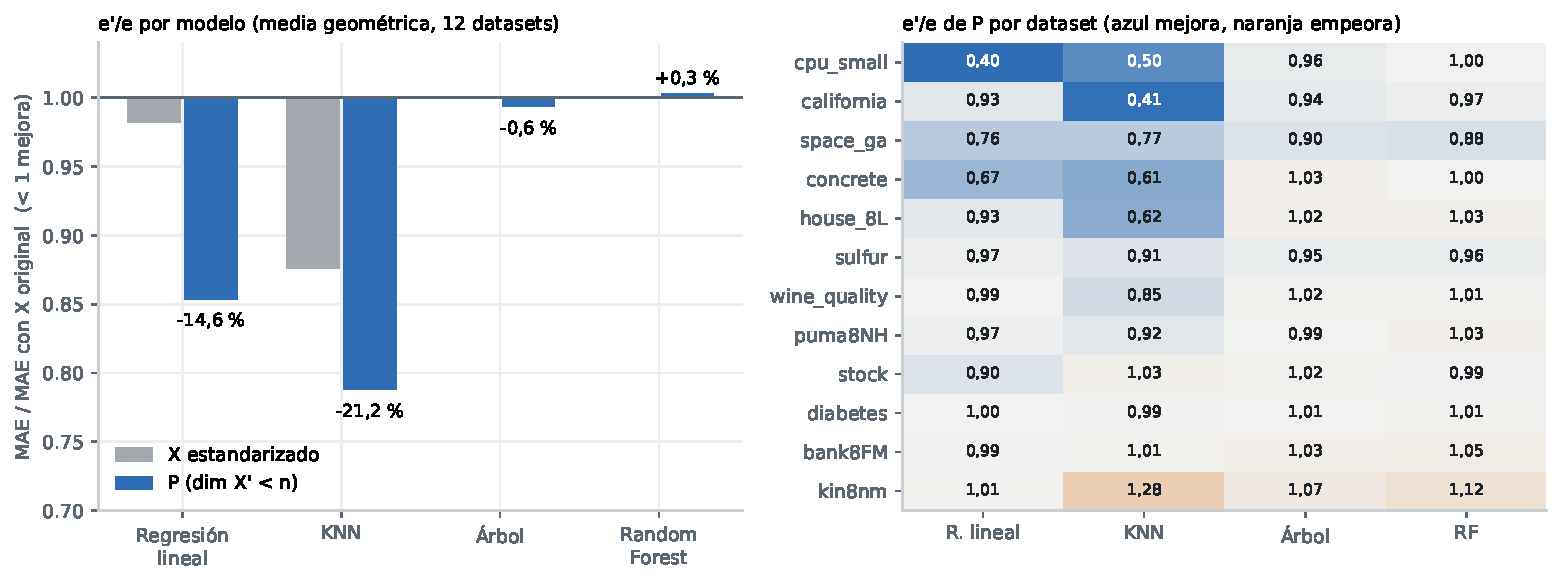
\includegraphics[width=0.84\textwidth]{principal}
\caption{Izquierda: $e'/e$ por modelo con $X$ estandarizado y con $X'=P(X)$. Derecha: $e'/e$ de $P$ por dataset
(azul: mejora; naranja: empeora).}
\label{fig:principal}
\end{figure*}
\begin{table}[t]\centering\footnotesize\setlength{\tabcolsep}{2.3pt}
\caption{$e'/e$ en las particiones de confirmación (media geométrica, 12 datasets). $p$: Wilcoxon por dataset con
Holm (8 contrastes), frente a $X$ original y frente a $X$ estandarizado.}
\label{tab:principal}
\begin{tabular}{@{}lcccccc@{}}\toprule
Modelo & estándar & $P$ & Datasets & $p$ & vs.\ est. & $p$\\\midrule
\filasPrincipal\bottomrule
\end{tabular}
\end{table}
Con $\dim X'<n$ (Tabla~\ref{tab:principal}, Fig.~\ref{fig:principal}), el MAE baja en \textbf{RL} un \cambioRL{}
(\dsRL{} datasets, $p=$\pRL), un \vsEstRL{} más que estandarizando, y en \textbf{KNN} un \cambioKNN{} (\dsKNN), un
\vsEstKNN{} más que estandarizando. Las mayores reducciones son \maxRL{} (\maxDsRL, RL; el MAE pasa de
\maxMaeOrig{} a \maxMaeP) y \maxKNN{} (\maxDsKNN, KNN). En el \textbf{árbol} (\cambioArbol) y \textbf{RF}
(\cambioRF) el error queda igual: un árbol no cambia con la forma ni con los pesos, y con menos de $n$ atributos solo
puede ganar si alguna dirección oblicua es mejor corte que el atributo original al que sustituye. KNN no es
significativo tras Holm por un único dataset, \peorDsKNN{} (\peorKNN): sus atributos importan todos por igual y
reducir obliga a perder información. Sin él (análisis de sensibilidad, no selección), KNN mejora \sinKinKNN{}
($p=$\pSinKinKNN) y la media de los cuatro modelos pasa de \cambioMedio{} a \sinKinMedio.

\subsection{Reducción y síntesis}
\begin{table}[t]\centering\footnotesize\setlength{\tabcolsep}{4pt}
\caption{$X'$ aprendida (media de 5 particiones): atributos originales y componentes conservados.}
\label{tab:dimension}
\begin{tabular}{@{}lcccc@{}}\toprule
Dataset & $n$ & originales & componentes & $\dim X'$\\\midrule
\filasDimension\bottomrule
\end{tabular}
\end{table}
$X'$ tiene siempre menos de $n$ atributos: de media \origMedia{} originales y \compMedia{} componentes, el
\dimMedia{} de $n$ (Tabla~\ref{tab:dimension}). La evolución elimina el \fracElim{} de los atributos originales y
conserva componentes en el \fracComp{} de las particiones: síntesis y reducción ocurren a la vez.

\subsection{Justificación de cada decisión}\label{sec:justificacion}
\begin{table}[t]\centering\scriptsize\setlength{\tabcolsep}{2.2pt}
\caption{Cribado de diseño (\cribCasos{} particiones de \emph{exploración}): $e'/e$ por modelo, media, peor modelo y
segundos por búsqueda.}
\label{tab:cribado}
\begin{tabular}{@{}lccccccc@{}}\toprule
Variante & RL & KNN & Árbol & RF & media & peor & s\\\midrule
\filasCribado\bottomrule
\end{tabular}
\end{table}
\textbf{Fitness} (Tabla~\ref{tab:cribado}). Con KNN solo, la $X'$ sirve sobre todo a KNN; con tres familias, la
media de los cuatro modelos mejora (\cribP{} frente a \cribKnn). Exigir que mejoren todos a la vez (minimax: el peor
modelo, cada uno relativo a sí mismo) empeora (\cribMinimax): el máximo de cuatro estimaciones ruidosas premia el
ruido. Aprender una $X'$ distinta para cada familia apenas mejora (\cribFamilia) y deja de ser una sola $X'$ para un
$M$ arbitrario. \textbf{Parada}: apartar un 20\,\% para parar ante el sobreajuste ahorra tiempo (\cribParadaSeg{}
frente a \cribPSeg\,s) pero empeora (\cribParada, \cribParadaTreinta{} con más paciencia, \cribSeleccion{} usando lo
apartado solo para elegir): quita datos al fitness para un criterio demasiado ruidoso.

\begin{table}[t]\centering\scriptsize\setlength{\tabcolsep}{2.2pt}
\caption{Ablación (\ablCasos{} particiones de confirmación): cambio del MAE frente a $P$ al cambiar una sola pieza
($>0$: peor que $P$; $^*$: $p<0{,}05$ por dataset con Holm) y $\dim X'/n$.}
\label{tab:ablacion}
\begin{tabular}{@{}lcccccc@{}}\toprule
Variante & RL & KNN & Árbol & RF & media & $d/n$\\\midrule
\filasAblacion\bottomrule
\end{tabular}
\end{table}
\textbf{Piezas} (Tabla~\ref{tab:ablacion}). Cambiar una sola pieza, en particiones de confirmación, muestra de dónde
viene la mejora. La \textbf{forma} es la que más aporta: sin ella ($\lambda=1$), RL empeora \ablSinFormaRL{}
(significativo). Con el \textbf{fitness solo de KNN}, KNN gana \ablKnnKNN{} pero RL pierde \ablKnnRL{}
(significativo): una sola $X'$ para un $M$ arbitrario necesita varias familias en el fitness. La \textbf{búsqueda
evolutiva} importa: con el mismo presupuesto, la búsqueda aleatoria empeora los cuatro modelos (\ablAleat{} de media;
RL \ablAleatRL, significativo). Un \textbf{AG} llega al mismo resultado que CMA-ES (\ablAG): cuenta buscar con
selección y variación más que el algoritmo concreto; se prefiere CMA-ES porque adapta sola la mutación, sin tasas
de cruce y mutación que fijar. \textbf{Sin el límite de $n-1$} el error no cambia de forma apreciable
(\ablSinLimite), pero $X'$ crece hasta \ablSinLimiteDim{}\,$n$: el límite garantiza la reducción que pide el
enunciado sin coste medible. \textbf{Sin síntesis} el error tampoco cambia (\ablSinSint): las componentes no dan una
mejora medible en estos datos, aunque la evolución las conserva en el \fracComp{} de las particiones; se mantienen
porque el enunciado pide síntesis y no empeoran nada.

\subsection{Comparativa con otras transformaciones}
\begin{table}[t]\centering\footnotesize\setlength{\tabcolsep}{2.2pt}
\caption{Comparativa en las particiones de confirmación: $e'/e$ (negrita: mejor; $^*$: $P$ mejor con $p<0{,}05$,
Wilcoxon por dataset con Holm), rango medio de Friedman (1 = mejor) y $d/n=\dim X'/n$.}
\label{tab:comparativa}
\begin{tabular}{@{}lcccccc@{}}\toprule
Transformación & R.\ lin. & KNN & Árbol & RF & Rango & $d/n$\\\midrule
\filasComparativa\bottomrule
\end{tabular}
\end{table}
Frente a estandarizar, Yeo-Johnson por máxima verosimilitud, cuantiles, ``solo PCA'' (95\,\% de varianza o \% por
validación cruzada), $X$ estandarizado con su PCA, MLKR (aprendizaje de métricas) y programación genética
(\texttt{gplearn}), $P$ tiene el \textbf{mejor rango medio} (\rangoP; Tabla~\ref{tab:comparativa}), y es la única que
mejora a RL y KNN a la vez \emph{reduciendo} la dimensión. La programación genética empata en RL pero usa $2n$
atributos, y ``solo PCA'', la otra forma de reducir, empeora a RF un \compPCARF: sustituir los ejes originales daña a
los árboles; \emph{elegir} cuáles conservar, no.

\section{Conclusiones}
\begin{itemize}
\item \textbf{$P$ cumple todos los requisitos}: solo entrenamiento, búsqueda evolutiva, síntesis y reducción
($\dim X'<n$ siempre, \dimMedia{} de media) con un criterio de eliminación que aprende CMA-ES.
\item \textbf{$e'<e$ en RL} (\cambioRL, significativo) \textbf{y KNN} (\cambioKNN), con hasta \maxRL{} y
\maxKNN; en los árboles el error queda igual.
\item \textbf{Mejor rango medio} entre nueve transformaciones, y la única que reduce mejorando RL y KNN.
\item \textbf{Cada decisión está contrastada}: el fitness de tres familias, la síntesis, la forma, el límite de
$n-1$ y CMA-ES frente a búsqueda aleatoria y un AG; la parada por sobreajuste se probó y se descartó.
\item \textbf{Límites}: 12 datasets pequeños y numéricos; un caso negativo (\peorDsKNN); la síntesis cumple el requisito pero no reduce el error de forma medible; los árboles no mejoran
porque lo que les ayuda es \emph{añadir} dimensiones; \segMediana\,s por búsqueda.
\end{itemize}
{\footnotesize\textbf{Reproducibilidad.} \texttt{ptca.py} (programa $P$ y estadística), \texttt{experimentos.py},
\texttt{analisis.py} y \texttt{notebook\_final.ipynb} (todo el proceso, ejecutable).\par}
\end{document}
